%!TeX encoding = utf8

% ------------------------------------------------------------------------------
% |                                 PRÉAMBULE                                  |
% ------------------------------------------------------------------------------

\documentclass[
	fontsize	= 11pt,
	twoside		= true
]{kaobook}

% Faux texte pour les tests
\usepackage{lipsum}


% --- Langues ------------------------------------------------------------------

\usepackage{polyglossia}
\setmainlanguage{english}
\setotherlanguage{french}

\usepackage{csquotes}


% --- Polices ------------------------------------------------------------------

\usepackage{fontspec}

\usepackage{fontawesome}


% --- Formatage ----------------------------------------------------------------



% --- Graphismes ---------------------------------------------------------------

\usepackage{tikz}

% Dossiers où chercher les graphiques
\graphicspath{{latexamu-intro/logo/}{graphismes/}}

% Formatage pour la page de garde AMU
% ------------------------------------------------------------------------------
% |                    FORMATAGE POUR LA PAGE DE GARDE AMU                     |
% ------------------------------------------------------------------------------

% --- Polices ------------------------------------------------------------------

\makeatletter
\newfontface\tit@el{Titillium-ExtraLight.ttf}[
	Path	= ./latexamu-intro/fonts/,
	Scale	= 1.1
]
\newfontface\tit@l{Titillium-Light.ttf}[
	Path	= ./latexamu-intro/fonts/,
	Scale	= 1.1
]
\newfontface\tit@m{Titillium-Regular.ttf}[
	Path	= ./latexamu-intro/fonts/,
	Scale	= 1.1
]
\newfontface\tit@sb{Titillium-SemiBold.ttf}[
	Path	= ./latexamu-intro/fonts/,
	Scale	= 1.1
]
\newfontface\tit@b{Titillium-Bold.ttf}[
	Path	= ./latexamu-intro/fonts/,
	Scale	= 1.1
]
\newcommand{\titel}[1]{{\tit@el #1}}
\newcommand{\titl}[1]{{\tit@l #1}}
\newcommand{\titm}[1]{{\tit@m #1}}
\newcommand{\titsb}[1]{{\tit@sb #1}}
\newcommand{\titb}[1]{{\tit@b #1}}

\newcommand\HUGE{\@setfontsize\Huge{28}{0}}
\makeatother

% --- Couleurs -----------------------------------------------------------------

\definecolor{blueamu}{RGB}{0, 101, 189}
\definecolor{cyanamu}{RGB}{61, 183, 228}

% --- Tikz ---------------------------------------------------------------------

\usetikzlibrary{decorations.markings}

\newcommand{\dhorline}[3][0]{%
    \tikz[baseline=-2pt]{\path[decoration={markings, 
      mark=between positions 0 and 1 step 2*#3
      with {\node[color=blueamu, fill, circle, minimum width=#3, inner sep=0pt, anchor=south west] {};}},postaction={decorate}]  (0,#1) -- ++(#2,0);}}
\newcommand{\dvertline}[3][0]{%
    \tikz[baseline=2em]{\path[decoration={markings,
      mark=between positions 0 and 1 step 2*#2
      with {\node[color=black!50, fill, circle, minimum width=#2, inner 
      sep=0pt, anchor=south west] {};}},postaction={decorate}] (0, #1) -- 
      ++(0,#3);}} 

% --- Divers -------------------------------------------------------------------

% Minipage de largeur variable
\usepackage{varwidth}



% --- Mathématiques ------------------------------------------------------------



% --- Bibliographie ------------------------------------------------------------



% --- Références croisées et métadonnées ---------------------------------------



% ------------------------------------------------------------------------------
% |                             CORPS DE LA THÈSE                              |
% ------------------------------------------------------------------------------

\begin{document}

% --- Pages de garde et mentions obligatoires ----------------------------------

\frontmatter

% Page de garde AMU

\begin{french}
\input{latexamu-intro/tex/titre}
\end{french}

\cleardoubleoddpage


% Attestation sous serment

\chapter*{Affidavit}
\input{latexamu-intro/tex/affidavit}

\cleardoubleoddpage


% Résumés

% En français
\begin{french}
\chapter*{Résumé}

\lipsum[1-4]

\bigskip

\textbf{Mots-clefs:} bla, bla, bla.

\end{french}

\cleardoubleoddpage

% ... et en anglais
\chapter*{Abstract}

\lipsum[1-4]

\bigskip

\textbf{Keywords:} blah, blah, blah.


\cleardoubleoddpage


% Publications liées à la thèse

\begin{french}
\chapter*{Publications et conférences}

\section*{Publications réalisées dans le cadre de la thèse}

% TODO utiliser un \printbibliography personnalisé


\section*{Participation aux événements scientifiques pendant la thèse}

\subsection*{Conférences}

\subsection*{Colloques}

\subsection*{Écoles de recherche}

\subsection*{Séminaires}

\end{french}

\cleardoubleoddpage


% --- Titres et introduction ---------------------------------------------------

\mainmatter
\pagelayout{wide}
\setchapterstyle{plain}


% Page de titre, version et licence

\title[Short title]{Title of the thesis}
\subtitle{Doctoral thesis in Mathematics}
\author{Prénom Nom}
\date{Publicly defended on \today}
\publishers{
	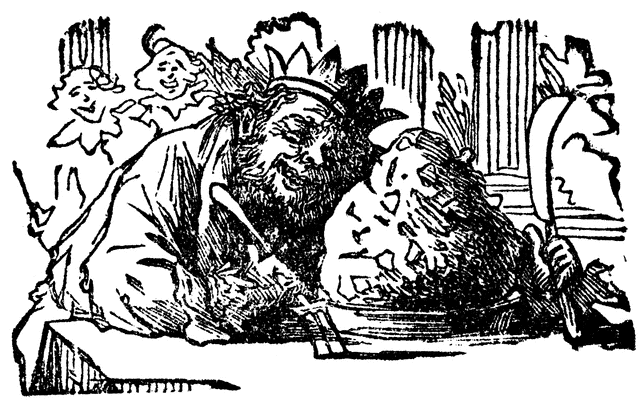
\includegraphics[width=7cm]{pudding1}
	\label{img:pudding1}
}

\uppertitleback{
	This is a draft from \today.
}

\lowertitleback{
	\faCreativeCommons{} \textbf{Prénom Nom 2022}
	\smallskip
	
	This work is distributed under the terms of the \href{https://creativecommons.org/licenses/by/4.0/}{Creative Commons Attribution 4.0 International Public License}. You are free to share and adapt it provided you give appropriate credit, provide a link to the license, indicate if changes were made, without suggesting the licensor endorses you or your use, nor further restrincting others from doing what the license permits.
}

\maketitle


% Remerciements
\addchap{Aknowledgements}


% Table des matières
\tableofcontents

\cleardoubleoddpage
\pagelayout{margin}
\setchapterstyle{kao}

% Introduction
\chapter{Introduction}

\lipsum[1-12]




% --- Partie 1 -----------------------------------------------------------------


% --- Annexes ------------------------------------------------------------------

\appendix

\backmatter

% Bibliographie
% -------------

% Index
% -----

% Colophon
% --------

\begin{french}
\vspace*{\fill}

\begin{center}
	Cette thèse a été composée avec \href{https://tug.org/xetex/}{\XeLaTeX}, pétulant rejeton de la lignée des \TeX. Elle utilise la délicieuse classe \href{https://github.com/fmarotta/kaobook}{\texttt{kaobook}} de Federico Marotta, basée sur le \href{https://github.com/kenohori/thesis}{travail} remarquable de Ken Arroyo Ohori, sur la classe \href{https://github.com/Tufte-LaTeX/tufte-latex}{Tufte-\LaTeX} et sur les infatigables outils \href{https://komascript.de/}{\KOMAScript}.
	
	Le \emph{pudding} du roi Arthur (page~\pageref{img:pudding1}) est issu du \href{https://etc.usf.edu/clipart/}{projet \emph{Clipart ETC}} de l'université de Sud-Floride.
\end{center}
\end{french}


\end{document}